\section{Results and evaluation}\label{sec:results}
All numbers in this section are generated from \file{results/}, from the evaluation measurements in \file{report/generated/eval\_plan.json} (\file{scripts/eval\_plan.py}) or from git, by \file{report/build\_report.py}. No case, parameter or seed was changed after seeing a result.

\subsection{The proposal's evaluation plan, row by row}
Table~\ref{tab:evalplan} takes each row of the proposal's evaluation plan (proposal Section~8) and says whether its ``done when'' criterion was met, with the evidence.

\begin{table}[ht]\centering\footnotesize
\caption{The proposal's evaluation plan against what was measured.}\label{tab:evalplan}
\begin{tabularx}{\textwidth}{@{}p{1.9cm}p{3.6cm}p{1.3cm}X@{}}
\toprule
\textbf{Check} & \textbf{Done when (proposal)} & \textbf{Met?} & \textbf{Evidence}\\
\midrule
Correctness & All fixtures match and every known equilibrium is found exactly. & Yes & \TestsCorrectness{} tests pass (\TestsFailedCorrectness{} fail): hand-computed judge fixtures, including a record that lands exactly on the clear-and-convincing bar; property tests (determinism, order independence, monotonicity, no single-item conviction); the solver on the prisoner's dilemma, battle of the sexes, matching pennies and rock-paper-scissors; a verifier that rejects non-equilibria.\\
Robustness & Every fixture gives its expected outcome; no crash or broken invariant; all replay hashes identical. & Yes, with one expectation not met as written & Four edge fixtures are library cases (Table~\ref{tab:edge}); every verdict is as expected, but in the defense-only fixture the Defender spent \DefenseOnlySpent{} budget units where the proposal expected none (the cost of the directed-verdict motion the Defender must now make, D5); the malformed case file and the illegal or out-of-turn action are tested as rejections (contract tests, the validator rule table, contempt after three violations). Fuzz: 100 generated cases $\times$ 25 pairings (Chaos and Mixed included) $=$ \StressTrials{} trials, \StressCrashes{} crashes, \StressInvariant{} broken invariants, and \StressReplays{} of \StressTrials{} replays identical. All \ReplaySame{} of \ReplayTotal{} recorded trials reproduce their pinned digest and \ReplayChain{} hash chains verify. \TestsRobustness{} tests in the robustness group pass.\\
Analysis & $4\times4$ payoff matrices over 200 common seeds per cell, with standard errors and 200 bootstrap resamples; each case labelled pure, mixed or dominance-solvable with the label's stability. & Yes, after a re-run & The first certified runs used \BootOldSeeds{} seeds per cell. We re-ran the payoff tables, the bootstrap and the classic-game labels at \BootSeeds{} seeds and \BootResamples{} resamples with the documented scripts (Table~\ref{tab:seeds}); Table~\ref{tab:bootstrap} gives each case's label and stability, and the stored payoff intervals bound each cell.\\
Sensitivity & Sanctions, costs, the scale 3 and each standard varied by $\pm25\%$; report which conclusions survive. & Yes, with fewer seeds & \SensVariations{} settings re-solved on \SensSeeds{} seeds per cell (fewer than the other analyses, to keep the run to minutes); \SensRobust{} cases never changed label, \SensFragile{} changed under at least one setting (Table~\ref{tab:sens}).\\
Live demo & Any case, pairing and seed stepped and replayed with the judge trace; a trial runs in under 1\,s, all six edge fixtures run cleanly live, and an examiner-made case never crashes the demo; works offline from a bundle. & Yes & Slowest of \TimedTrials{} timed pairings: \TrialMaxMs{}\,ms (median \TrialMedianMs{}\,ms). The four edge cases play live; the other two fixtures are input rejections. \TestsLiveDemo{} tests of the API, the CLI, the editor and the recorded bundle pass, including absurd editor input (empty, huge, negative, non-numeric and script-tag values) typed into a real browser. The bundle makes the demo run offline.\\
\bottomrule
\end{tabularx}
\end{table}

\begin{table}[ht]\centering
\caption{The four edge fixtures that are library cases, as measured (Bold against Careful, seed 0). The proposal fixed the expected outcome before any code: the empty docket and the defense-only case end at the directed-verdict review (DV-2) with the Defender winning, (the proposal also expected the Defender to spend nothing in the defense-only case; it spent the cost of the motion, see Table~\ref{tab:evalplan}); two equally credible, mutually exclusive witnesses cancel and the burden of proof decides for the Defender; and when every exhibit is defective, each objected exhibit is excluded and its presenter sanctioned, and the verdict equals the verdict on the admitted record.}\label{tab:edge}
% generated by report/build_report.py: do not edit
{\footnotesize
\begin{tabularx}{\textwidth}{@{}>{\raggedright\arraybackslash}p{3.7cm}>{\raggedright\arraybackslash}p{3cm}>{\raggedright\arraybackslash}p{4.6cm}>{\raggedright\arraybackslash}p{2.6cm}@{}}
\toprule
\textbf{Edge fixture} & \textbf{Verdict (Bold vs Careful, seed 0)} & \textbf{Rules fired} & \textbf{Budget spent (Accuser / Defender)} \\
\midrule
edge-defense-only & directed acquittal & DV-2, ELEM-1, STD-1, VER-DV & 0 / 0.5 \\
edge-empty-docket & directed acquittal & DV-2, ELEM-1, STD-1, VER-DV & 0 / 0.5 \\
edge-mutual-exclusion & not liable & ADM-WAIVER, DV-2, ELEM-1, OBJ-HEARSAY, SANCTION-OVR, STD-1 & 2 / 1.5 \\
edge-poisoned-tree & not guilty & ADM-WAIVER, DV-2, ELEM-1, OBJ-AUTH, OBJ-DISCLOSURE, OBJ-EXCLUSIONARY & 5.5 / 2 \\
\bottomrule
\end{tabularx}}

\end{table}

Two proposal items were stretch goals: replicator dynamics (implemented in \file{gametheory/dynamics.py}) and an expectimax agent (replaced by a depth-limited alpha-beta \emph{lookahead} lawyer that weighs an opponent's objection by its own belief; an exhibition, not certified). The hash-chained log and the terminal replay (\texttt{python -m courtroom run}) were kept.

\subsection{Does strategy matter here?}
Table~\ref{tab:matters} and Figure~\ref{fig:matters} measure, for each case, how far the lawyers' styles and the seed move the Accuser's win rate (\MSeeds{} seeds, all nine pairings of Bold, Careful and Smart). The lawyers move the verdict in \NMove{} of \NCases{} cases (\NLawyers{} decided by the lawyers and \NPartly{} partly); the other \NEvidence{} are decided by the evidence alone, so in those no style and no seed changes the verdict and a strategy comparison has nothing to find. This was the first thing we measured and it was uncomfortable: it is why the demo script names which cases to use to show strategy mattering and which to present as plain trials.

\begin{table}[ht]\centering\caption{Does strategy matter? (Generated from \file{results/matters.json} and \file{matters\_surprises.json}.)}\label{tab:matters}
% generated by report/build_report.py: do not edit
{\small
\begin{tabularx}{\textwidth}{@{}>{\raggedright\arraybackslash}p{4cm}>{\raggedright\arraybackslash}p{2.9cm}rr>{\raggedright\arraybackslash}p{2.9cm}@{}}
\toprule
\textbf{Case} & \textbf{Verdict (plain rules)} & \textbf{Lawyers move it by} & \textbf{Seed coin-flip} & \textbf{Verdict (surprises on)} \\
\midrule
Aurora Protocol Flash-Loan Exploit & Decided by the evidence & 0\% & 0\% & Decided by the evidence \\
The Broken Bike & Decided by the lawyers & 50\% & 22\% & Partly the lawyers \\
The Missing Cookies & Decided by the evidence & 0\% & 0\% & Decided by the evidence \\
Prosecution Brings Only Exculpatory Material & Decided by the evidence & 0\% & 0\% & Decided by the evidence \\
The Empty Docket & Decided by the evidence & 0\% & 0\% & Decided by the evidence \\
Mutually Exclusive Testimony & Decided by the evidence & 0\% & 0\% & Decided by the evidence \\
Fruit of the Poisonous Tree & Partly the lawyers & 25\% & 17\% & Partly the lawyers \\
The Dug-Up Garden & Decided by the evidence & 0\% & 0\% & Decided by the evidence \\
Helix Dynamics Trade-Secret Exfiltration & Decided by the lawyers & 100\% & 17\% & Decided by the lawyers \\
AV-7 Crosswalk Collision & Decided by the lawyers & 100\% & 8\% & Decided by the lawyers \\
\bottomrule
\end{tabularx}}

\end{table}
\begin{figure}[ht]\centering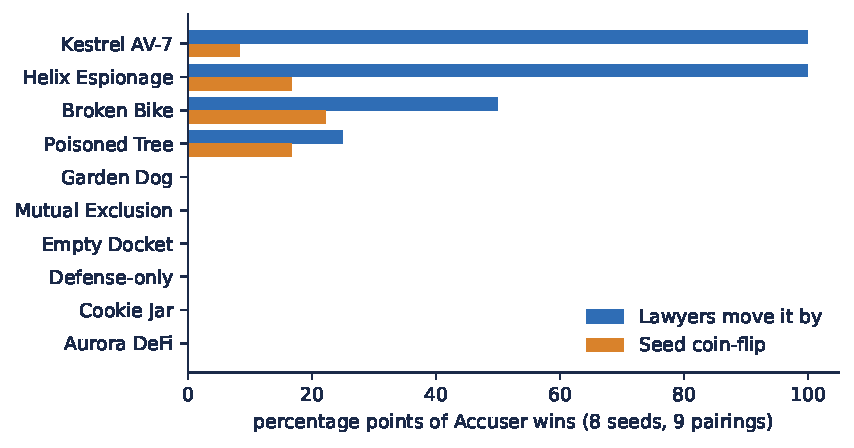
\includegraphics[width=0.78\textwidth]{figures/fig_matters.pdf}\caption{How far the lawyers and the seed move the Accuser's win rate in each case (plain rules).}\label{fig:matters}\end{figure}

\subsection{How stable are the equilibrium labels?}
Each game was re-solved on \BootResamples{} resamples of \BootSeeds{} seeds (Table~\ref{tab:bootstrap}, Figure~\ref{fig:bootstrap}). With plain rules, \BootBelowPlain{} cases came back less than $80\%$ of the time; the lowest is \BootWorstPlainCase{} at \BootWorstPlain{}. With courtroom surprises on, \BootBelowSurprises{} case falls below $80\%$: \BootWorstSurprisesCase{} at \BootWorstSurprises{}.

The earlier run at \BootOldSeeds{} seeds looked weaker: \BootOldBelow{} cases were below $80\%$ under plain rules (\BootOldWorstCase{}, \BootOldWorst{}; \BootOldSecondCase{}, \BootOldSecond{}). Doubling the seeds raised those, which suggests the weak stability at \BootOldSeeds{} seeds was partly sampling noise. We report both runs because the earlier one is in the git history (Section~\ref{sec:discussion}).

\begin{table}[ht]\centering\caption{Equilibrium label and its bootstrap stability.}\label{tab:bootstrap}
% generated by report/build_report.py: do not edit
{\small
\begin{tabularx}{\textwidth}{@{}>{\raggedright\arraybackslash}p{5cm}lrlr@{}}
\toprule
\textbf{Case} & \textbf{Label (plain)} & \textbf{Stability} & \textbf{Label (surprises on)} & \textbf{Stability} \\
\midrule
Aurora Protocol Flash-Loan Exploit & pure & 100.0\% & pure & 100.0\% \\
The Broken Bike & mixed & 87.0\% & pure & 83.0\% \\
The Missing Cookies & pure & 100.0\% & dominance-solvable & 100.0\% \\
Prosecution Brings Only Exculpatory Material & pure & 100.0\% & pure & 100.0\% \\
The Empty Docket & pure & 100.0\% & pure & 100.0\% \\
Mutually Exclusive Testimony & pure & 100.0\% & pure & 100.0\% \\
Fruit of the Poisonous Tree & mixed & 100.0\% & mixed & 100.0\% \\
The Dug-Up Garden & pure & 100.0\% & pure & 60.5\% \\
Helix Dynamics Trade-Secret Exfiltration & mixed & 99.5\% & mixed & 100.0\% \\
AV-7 Crosswalk Collision & mixed & 97.5\% & dominance-solvable & 88.5\% \\
\bottomrule
\end{tabularx}}

\end{table}
\begin{figure}[ht]\centering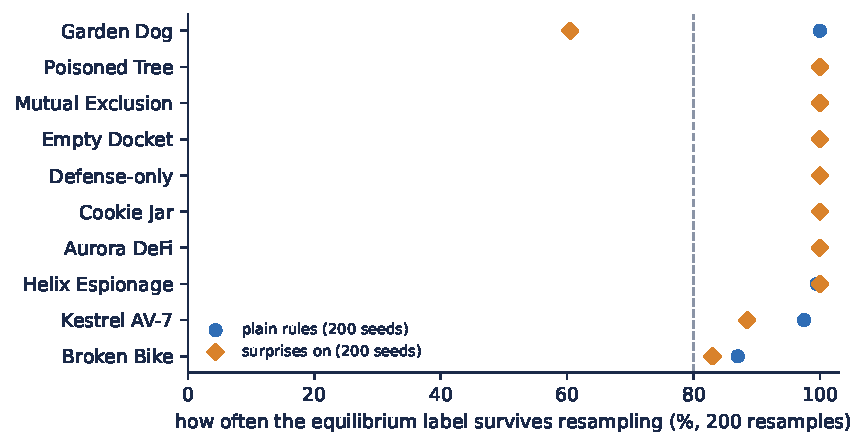
\includegraphics[width=0.78\textwidth]{figures/fig_bootstrap.pdf}\caption{Bootstrap stability of each case's equilibrium label; the dashed line is $80\%$.}\label{fig:bootstrap}\end{figure}

\subsection{Does the rulebook's choice of constants decide the conclusions?}
Table~\ref{tab:sens} counts how many cases changed label when each constant was moved. The constant that changes most labels is the prior defect rate (\SensPriorChanges{} label changes), the lawyers' prior that any ground applies to an exhibit; this is a belief inside the agents, not a rulebook constant, and it is a modelling choice we did not measure.

\begin{table}[ht]\centering\caption{Label changes under the sensitivity sweep.}\label{tab:sens}
% generated by report/build_report.py: do not edit
{\small
\begin{tabularx}{\textwidth}{@{}lrr@{}}
\toprule
\textbf{Constant moved} & \textbf{Label changes (plain)} & \textbf{Label changes (surprises on)} \\
\midrule
LLR SCALE & 1 & 2 \\
PRIOR DEFECT RATE & 6 & 6 \\
beyond reasonable doubt & 1 & 2 \\
costs & 1 & 2 \\
sanctions & 1 & 3 \\
standards of proof & 0 & 0 \\
\bottomrule
\end{tabularx}}

\end{table}

\subsection{Can a better lawyer be found?}
The best-response search found a lawyer that beats the four hand-written styles in \NBeaten{} of \NSearches{} searches (each searched case is run with surprises off and on); the largest gain is \BestGain{} utility per trial for the Defender in \BestCase{} with plain rules. Every kept profile was confirmed on seeds that played no part in finding or accepting it (Table~\ref{tab:oracle}, Figure~\ref{fig:oracle}). ``No better lawyer found'' means none was found in a five-parameter family within a budget of \OracleBudget{} profiles per side per round; it is evidence, not proof.

\begin{table}[ht]\centering\caption{Best-response search results.}\label{tab:oracle}
% generated by report/build_report.py: do not edit
{\small
\begin{tabularx}{\textwidth}{@{}>{\raggedright\arraybackslash}p{4.9cm}lrr>{\raggedright\arraybackslash}p{3.5cm}@{}}
\toprule
\textbf{Case} & \textbf{Surprises} & \textbf{Kept} & \textbf{Confirmed on fresh seeds} & \textbf{Gain per trial vs the old equilibrium} \\
\midrule
The Broken Bike & off & 1 & 1 of 1 & defense: +0.88 \\
The Broken Bike & on & 0 & 0 of 0 & none \\
Helix Dynamics Trade-Secret Exfiltration & off & 2 & 2 of 2 & defense: +1.59 \\
Helix Dynamics Trade-Secret Exfiltration & on & 2 & 2 of 2 & defense: +0.91 \\
AV-7 Crosswalk Collision & off & 0 & 0 of 0 & none \\
AV-7 Crosswalk Collision & on & 1 & 1 of 1 & prosecution: +1.22 \\
\bottomrule
\end{tabularx}}

\end{table}
\begin{figure}[ht]\centering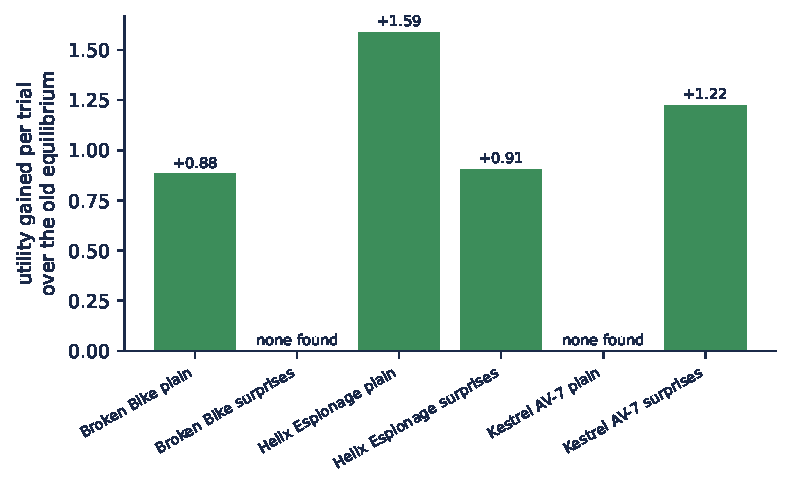
\includegraphics[width=0.78\textwidth]{figures/fig_oracle.pdf}\caption{Utility gained per trial by the best discovered lawyer over the old equilibrium.}\label{fig:oracle}\end{figure}

\subsection{The lecture concepts, computed on our own games}
Table~\ref{tab:lectures} lists each lecture concept, what our data says and the relaxation or limit it carries. Of the games the brief named, none of the prisoner's dilemma, stag hunt, battle of the sexes or chicken was found among the \ClassicCorners{} two-by-two corners of the library (\ClassicFoundTotal{} found), and \SearchKept{} survived the search over \SearchTried{} generated cases: \SearchLookedDilemma{} corners looked like a prisoner's dilemma and \SearchLookedStag{} like a stag hunt when read as exact numbers, but none kept its name under the full tolerance on fresh seeds. Matching pennies appears in \MatchingPennies{} corners. The minimax theorem held in \TheoremHolds{} of \TheoremTotal{} win-probability games. The trial tree was solved exactly in \TreeSolved{} of \TreeTotal{} cases and plain minimax, alpha-beta and alpha-beta with move ordering agreed in every one (Figure~\ref{fig:tree}). The lookahead lawyer beat the four-style equilibrium in \LookBeats{} of \NCases{} cases (\LookBeatsCase{}). ``Not found'' is a statement about the library and the cases tried, not a proof that no such case exists; no case was retuned to make a classic game appear.

\begin{table}[ht]\centering\caption{Lecture concepts: where each is computed and what our data says (generated).}\label{tab:lectures}
% generated by report/build_report.py: do not edit
{\footnotesize
\begin{tabularx}{\textwidth}{@{}>{\raggedright\arraybackslash}p{2.8cm}>{\raggedright\arraybackslash}p{5.2cm}>{\raggedright\arraybackslash}p{6cm}@{}}
\toprule
\textbf{Lecture concept} & \textbf{What our data says} & \textbf{Relaxation or limit} \\
\midrule
Prisoner's dilemma & \textbf{Not found.} 0 of 360 corners in the library, and 0 kept after searching 395 generated cases. & Only pairs of styles (2×2 corners of the 4×4 table). A gap under two standard errors is a tie, and a game needing a strict order where there is a tie is called none of the classic games. \\
Stag hunt & \textbf{Not found.} 0 of 360 corners in the library, and 0 kept after searching 395 generated cases. & Risk is read from each play's worst case (a security-level notion), not from risk dominance. \\
Battle of the sexes (Bach or Stravinsky) & \textbf{Not found.} 0 of 360 corners in the library, and 0 kept after searching 395 generated cases. & Needs two pure equilibria that the sides rank differently. \\
Chicken & \textbf{Not found.} 0 of 360 corners in the library, and 0 kept after searching 395 generated cases. & The same two-equilibria shape with a full strict order of four outcomes. \\
Matching pennies & 16 corners (plain), 14 (surprises on) & Named when no pure equilibrium survives the tolerance; the sides need not be zero-sum. \\
Pareto optimality & Some equilibrium dominated for both sides in 1 of 10 cases (plain), 1 (surprises on). & Compared on mean payoffs over pure pairs of styles; a mixed equilibrium is compared by its expected payoffs, and mixing across cells together is not considered. \\
Minimax and the minimax theorem & Maximin = minimax = Nash value in 20 of 20 win-probability games. & Holds only for the constant-sum win-probability game. The real game is general-sum, so there the security value is only a floor. \\
Minimax on the trial tree & 17 of 18 cases solved exactly. & An open-file relaxation: both sides see all exhibits and flaws, no perception noise, and a zero-sum payoff (Accuser utility minus Defender utility). The real game has hidden information and is not zero-sum. \\
Alpha-beta pruning & Same value as plain minimax in all 15 cases where both finished, with move ordering cutting the nodes visited as shown in the table. & Pruning is exact; the saving depends on the case and on the ordering heuristic. \\
Thinking ahead (depth-limited alpha-beta) & Beat the four-style equilibrium in 1 of 10 cases (plain) and 1 (surprises on). & Exhibition, not certified. It uses only its own view and the public oracle, assumes the worst reply, and scores positions with a heuristic. \\
\bottomrule
\end{tabularx}}

\end{table}
\begin{figure}[ht]\centering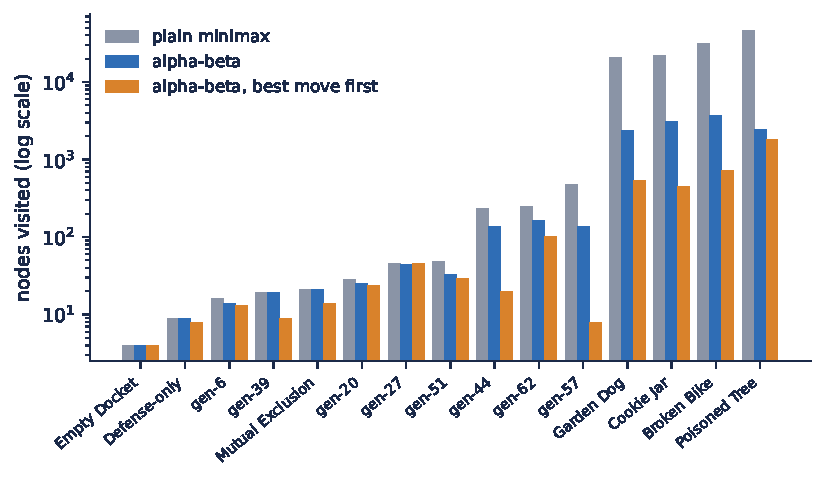
\includegraphics[width=0.85\textwidth]{figures/fig_tree.pdf}\caption{Nodes visited by plain minimax, alpha-beta and alpha-beta with move ordering on the cases where all three finished (log scale).}\label{fig:tree}\end{figure}

\subsection{An example payoff table}
Figure~\ref{fig:payoff} shows the Accuser's win rate for each pair of styles in one case where the lawyers matter. The equilibrium of such a table is what the analyses above label.

\begin{figure}[ht]\centering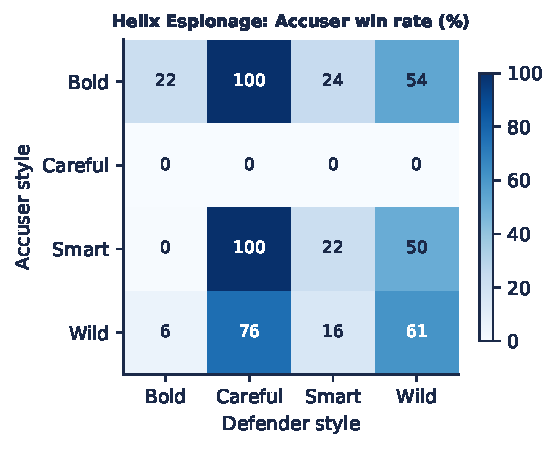
\includegraphics[width=0.5\textwidth]{figures/fig_payoff.pdf}\caption{The Accuser's win rate (\%) for every pair of the four styles in a case the lawyers decide (\BootSeeds{} seeds per cell).}\label{fig:payoff}\end{figure}

\subsection{Seeds per cell actually used}
\begin{table}[ht]\centering\caption{Seeds per cell, read from the result files.}\label{tab:seeds}
% generated by report/build_report.py: do not edit
{\small
\begin{tabularx}{\textwidth}{@{}>{\raggedright\arraybackslash}p{6cm}>{\raggedright\arraybackslash}p{5cm}r@{}}
\toprule
\textbf{Analysis} & \textbf{File} & \textbf{Seeds per cell} \\
\midrule
Bootstrap of the equilibrium label & \texttt{results/bootstrap.json} & 200 \\
Classic-game labels & \texttt{results/classic.json} & 200 \\
Pareto and security & \texttt{results/efficiency.json} & 200 \\
Rulebook sensitivity & \texttt{results/sensitivity.json} & 16 \\
Does strategy matter & \texttt{results/matters.json} & 8 \\
Lookahead comparison & \texttt{results/lookahead.json} & 40 \\
\bottomrule
\end{tabularx}}

\end{table}
